\section{Single particle modes of heat transfer}

\begin{figure}[t]
	\centering
	\caption{Each ceramic pebble in a fusion reactor will experience multiple modes of heat transfer.}
	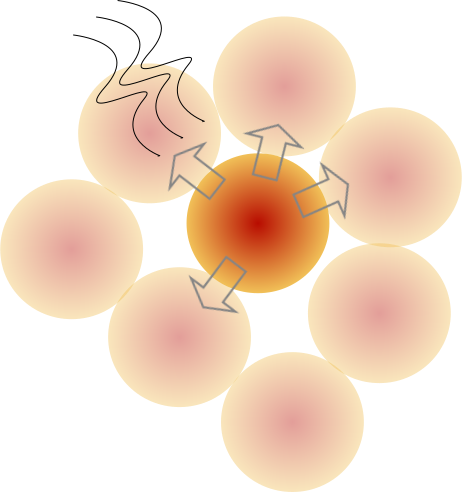
\includegraphics[width=0.75\textwidth]{chapters/figures/pebble-complete-heat-transfer}\label{fig:peb-comp-ht}
\end{figure}

The transient energy balance for an irradiated pebble, shown in Fig.~\ref{fig:peb-comp-ht}, in a packed bed with flowing interstitial gas is given by Eq.~\ref{eq:single-pebble-energy},

\begin{equation}\label{eq:single-pebble-energy}
	\rho V C \frac{\mathrm{d}T}{\mathrm{d}t} = \dot{Q}_g + Q_\text{conduction} + \dot{Q}_\text{convection} + \dot{Q}_\text{radiation}
\end{equation}

We begin with the lumped capacitance assumption that internal temperature gradients inside of the solid particle are negligible thus we can neglect diffusion terms in the solid. The validity of that assumption for the ceramic pebbles in fusion reactors will be discussed in detail in \S\ref{sec:ht-jeffreson-correction}. The terms on the right-hand-side of Eq.~\ref{eq:single-pebble-energy} are:

\begin{enumerate}
\item rate of energy generated internal to the pebble,
\item rate of conduction between neighboring pebbles in their regions of contact, 
\item rate of convective heat transfer with the interstitial helium gas (which includes energy carried far downstream or redeposited to neighboring pebbles), and
\item rate of radiative exchange between local solids.
\end{enumerate}

In this section we will provide a brief overview of all the modes of heat transfer to provide an overview of the importance and impact of each mode. For cases when more detail is needed, the details will be expounded in their own complete sections.

\subsection{Heat generation}

Nuclear deposition of energy is handled in a straightforward manner. With a known volumetric energy generation rate, $q'''$ prescribed by, for instance, the neutron heating in the volume, the heat generation rate for this particle is simply

\begin{equation}
	\dot{Q}_g = q'''V
\end{equation}



\subsection{Conduction with neighboring particles}

When the particle is in contact with neighboring particles of differing temperature, they will transfer energy via conduction. If we begin by considering just two isothermal particles, we may employ a heat conductance term, $h_c$, to generically quantify the ease of energy movement between the two particles. In that case, the rate of heat transferred between the particles is written as

\begin{equation}
	\dot{Q}_\text{conduction, 1-2} = h_c(T_1 - T_2)
\end{equation}

where the heat conductance has units of \si{W/K}, not to be confused with the units of the heat transfer coefficient employed in convective heat trasnfer. Obviously this same term may be applied to all contacting neighbors such that the total rate of energy transfer due to conduction can be generically written as

\begin{equation}
	\dot{Q}_\text{conduction} = \sum_{\forall \text{contacts}} \dot{Q}_\text{conduction,1-contact}h_c(T_1 - T_\text{contact})
\end{equation}

Of course, we must be careful with the application of this summation. We are assuming that a particle's interaction with each neighbor proceeds indepedently and thus their results can be superimposed. Furthermore, we have not given a means of calculating the heat conductance, $h_c$. These issues will be addressed more completely in \S\ref{sec:particle-conduction}. 



\subsection{Convection by interstitial gas}

Engineers have paid considerable attention to the calculation of convective heat transfer in packed beds. Correlations for determining the Nusselt number of a sphere in dilute and dense packings over a range of Reynolds and Prandtl number are available. We will cover the detail of many of these correlations in \S\ref{sec:}. The methods all come down to calculating Nusselt number to find the heat transfer coefficient and then computing the rate of heat transfer from convection as

\begin{equation}
	\dot{Q}_\text{convection} = -hA(T_s-T_f)
\end{equation}

where $T_s$ is the temperature of the solid with surface area, $A$, and $T_f$ is the average bulk temperature of the passing fluid. The negative sign is to maintain convention that energy transfer into the solid is positive.





\subsection{Radiative transfer with neighboring particles}

The radiation exchange between contacting neighbors becomes excessively complex in a packed bed due to the local and semi-local nature of radiation. A standard approach to radiation exchange between surfaces is to consider the view factor between them. In a dense, randomly packed bed of spheres the computation of view factors between pebbles can be done via a method such as that proposed Feng and Han\cite{Feng2012}. 
